\documentclass[a4paper]{article}
\usepackage[utf8]{inputenc}
\usepackage{graphicx}

\begin{document}

\section{Vererbung}

Gregor Mendel (1822 - 1884) war zuständig für den Klostergarten (Mönch). Er hat zufällig Erbsen in verschiedenen Farben gepflanzt. Er hat nun verschiedene Farben miteinander gekreuzt, um zu sehen was passiert.
\newline
\newline
Unformitätsregel:
\newline
\newline
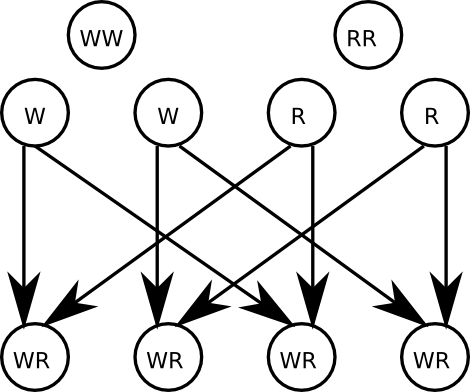
\includegraphics[scale=0.25]{image/1.png}
\newline
\newline
Spaltungsregel:
\newline
\newline
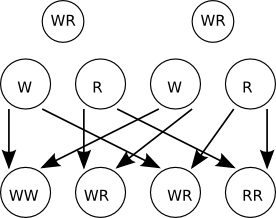
\includegraphics[scale=0.75]{image/2.png}
\newline
\newline
Die Kinder von reinrassingen Eltern sind Mischlinge. Genotypus sind alle gespeicherten Merkmalen in der Zelle. Phenotypus sind alle ausgebildeten Merkmale. Merkmale können rezessiv oder dominat sein. Dominante Merkmale setzten sich bei Kreuzungen mit rezessiven Merkmale durch und werden ausgebildet. Die Körperzelle hat alle Merkmale doppelt gespeichert (nennt man Diploid). Die Geschlechtszellen haben die Merkmale nur einmal gespeichert (nennt man Happloid).
\newline
\newline
Die Bluterdkrankheit kann sich bei Inzucht besonders gut weiterbilden. Der Mann erkrankt jedoch leichter als die Frau, da Männer (XY Chromosom) schon erkrankt sind wenn das X die Krankheit hat. Bei der Frau (XX Chromosom) müssen beide X-Chromosome erkrankt sein, damit die Frau die Krankheit hat.

\newpage

\section{Zellteilung}

Die Zellteilung wird auch Mitose genannt (normale Körperzellteilung). Zellen enstehen nur durch die Teilung von Körperzellen.

\subsection{DNS - Desoxyribonukleinsäure}

Die DNS kann sich vervielfältigen, denn bevor die Zellteilung beginnt muss sich die DNS mit den Erbinformationen kopieren.
\newline
\newline
Die DNS besteht aus vielen Chromosomen (bei Menschen sind es 48). Das Wort Chromosomen stammt aus dem Lateinischen und man versteht darunter "Farbkörper".
\newline
\newline
Aufbau der DNS:
\newline
\newline
Die DNS ist besteht aus einen Doppelstrang und jeder Strang besteht aus Tripplets. Ein Tripplet sind drei Basen. Viele Tripplets bilden eine Aminosäure (=Eiweiß). Viele Eiweiße sind ein Gen und viele Gene ist ein Chromosom und viele Chromosome bilden die DNA. 
\newline
\newline
Es gibt vier verschiedene Basen:
\newline
\newline
\begin{itemize}
\item Adenin
\item Thymin
\item Guanin
\item Cytosin
\end{itemize}

Bei der Zellteilung muss die DNS vollständig kopiert werden, dabei öffnet sich der Doppelstrang und durch Anlieferung und Ablagerung entsprechender Basen werden aus einem Doppelstrang zwei Doppelstränge $\rightarrow$ entspricht der identen Kopie der Chromosomen. Eine plötzlich spontane Änderung der Erbinformation durch Kopierfehler oder anderen Ursachen (Energiereiche Strahlung, Chemikalien) nennt man Mutation (99,99\% alle Mutationen sind negativ behaftet, die positiven Mutationen sind mit Triebfehler für die Evolution behaftet).

\newpage

\section{Makromoleküle}

Makromoleküle (Riesenmoleküle) sind sehr große Moleküle, die aus sich wiederholenden, gleichen oder unterschiedlichen Struktureinheiten (formale Grundbausteine) bestehen.

\subsection{Kohlenhydrate}

Kohlenhydrate sind Großmoleküle, die entstehen bei aneinanderreihen von Zucker, z.B. Monosaccharide (Einfachzucker).
\newline
\newline
Glukose (ein Einfachzucker) C6H12O6
Ribose ist ein Zucker mit fünf C-Atomen (5-Ring)
Fructose C6H12O6
\newline
\newline
Rohr- und Rübenzucker ist ein Zweifachzucker (Saccharose), der je aus einem Fructose Molekül und einem Glucose  Molekül bestehen.
\newline
\newline
Polysaccheride sind Mehrfachzucker und bestehen aus vielen Zuckermolekülen.
Amylose sind unverzweigte Ketten mit 60 bis 300 Zuckermolekülen.
Amyloptektin sind verzweigte Ketten mit 300 bis 1000 Zuckermolekülen.
Zellulose sind unverzweigte Ketten bis zu 5000 Zuckermoleküle (ist in allen Pflanzen enthalten). Pflanzen bilden Zellulose (kann gewonnen werden).

\subsubsection{Fotossyntese}

Unter Fotossyntese versteht man die Zuckerproduktion der Pflanzen durch Sonnenlich.

n*CO2 + n*H20  $\rightarrow$ (Katalysator: Chlorophyl) C6H12O6 (Glukose) + n*O (Sauerstoff wird frei)

Was passiert mit dem Sauerstoff und Zucker? - Wie viel Sauerstoff die Pflanze abgibt entscheidet sie selbst. Sie verwendet den Sauerstoff und Zucker als Baustoff für sich selbst (z.B. Zellulose, Holz). Wenn die Pflanze wächst hat sie gut gewirtschaftet. Die Pflanzen verbrauchen in der Nacht ihren Sauerstoffvorrat.

\subsection{Eiweiße (=Proteine)}

Eiweiße sind in der Biologie sehr wichtig. Ihre Aufgabe ist es irgendwas zu ''regeln''. Proteine oder Eiweiße sind aus Aminosäuren aufgebaute biologische Makromoleküle.
\newline
\newline
Grundstruktur ist nicht kompliziert:
\newline
\newline
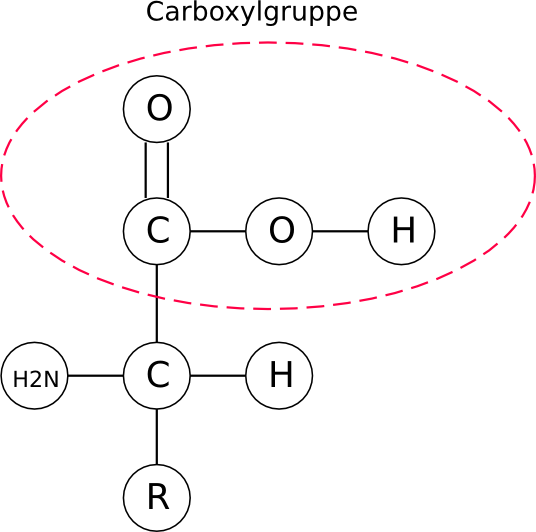
\includegraphics[scale=1]{image/3.png}
\newline
\newline
R ... Rest (z.B. Aminubutonsäure)
\newline
\newline
\subsubsection{Aufgaben der Proteine}

\begin{itemize}
\item Enzymatische Katalysator (Enzyme $\rightarrow$ Biokatalysator), viele Vorgänge im menschlichen Körper werden über Proteine / Eiweiß geregelt; Vitamine sind Enzyme, die nicht vom Körper selber produziert werden können

\item Transport: Hemoglobin $\rightarrow$ Transportstoffe für Sauerstoff (Eisen)

\item Bewegung: Proteine sind Hauptbestandteil des Muskelgewebes

\item Mechanische Stückfunktion: Kolagene; geben der Haut und Sehnen ihre Reißfestigkeit

\item Immunsystem: Antikörper sind hochspezialisierte  Proteine, die Fremdsubstanzen wie Viren, Bakterien oder Fremdzellen erkennen und binden können (Weißen Blutkörper); Bakterien vergiften; Viren zerstören Zellen; Fremdkörper können Krankheiten übertragen

\end{itemize}

\subsection{Fette}

Fette und fette Öle sind Ester des dreiwertigen Alkohols Glycerin mit drei, meist verschiedenen, Monocarbonsäuren, den Fettsäuren (Ester bedeutet eine Verbindung zwischen organischen Säuren und Alkhol (z.B. Propantriol bzw. Glyzerin und Methansäure).
\newline
\newline
Propantriol + Methansäure (Ameisensäure) = Fett

\newpage

\section{Gesundheit}

Richtige Ernährung

Ernährung heißt Energie zuführen. 
Energie kann auf verschiedene Form - in chemischer Form zugeführt werden
die Stoffe haben einen bestimmten Joule Wert 1k Kalorie = 4,2k Joule

Jetzt ist es so das man als ausgeachsenen mensc einen bestimmten joule verbraucht. weil es den betriebswert gi bt endoterm es muss energie zugeührt werden zusätlich kommt ein teil dazu wenn man aktiv ist (bewegung) 

Der Grundbedarf ist der Bedarf an Energie, die ein Mensch beim Sitzen oder Liegen verbraucht. Der Grundumsatz (=Grundbedarf) bei einem 70 Kilo Menschen ist in etwa 7000k Joule. Tätigkeitsumsatz kann bis zu 20000k Joule zusätzlich brauchen.

Der Mensch ist ein Heterotropher, der Mensch ist ein Allesfresser. Der Fettanteil sollte 25\% der Eingenommen Essen (hängt vom Verbrauch aus). Vitamine sind Stoffe, die der Körper nicht alleine herstellen kann.

Wichtige Vitamine:

\begin{itemize}
\item Vitamin A (Retinol)
\item Vitamin B1 (Thiamin)
\item Vitamin B2-Gruppe 
\item Vitamin B6 (Pyridxoin)
\item Vitamin B12 (Cobalamin)
\item Vitamin C
\item Vitamin D
\item Vitamin E (Fruchtbarkeisvitamin)
\item Vitamin K
\end{itemize}

\section{Krankheiten durch falsche Ernährung}

Der Zuckergehalt wird über Insoline
Bauchspeicheldrse Insoline, Nebennieren Hypophyse 

\section{Gicht}

Harnssäurespiegel im Blut is zu groß und diese Harnsäure lagert sich in den gelenken an den schleimbeuteln und sehnen ab, Ursache ist das Burin, die kommt in tierischen Nahrungsmittel (Innerein,, Hüllsenfrüchte). Sehr schmerzhaft. Hizegefühl. 

\section{Fettsucht}

Überschreitung des Normal Gewichts [kg/(Größe)^2]. 

\begin{itemize}
\item Zuckerkrankheit 
\end{itemize}

\section{Hormone}

Sind Stoffe, die der Körper selber herstellen kann.
\end{document}